\begin{quote}
    \textit{``You might not be familiar [with these topological concepts]. But you need to get familiar because we're going to squeeze physics out of this like there's no tomorrow.'' --Jorge Santos}
\end{quote}
We continue our discussion of focusing of geodesics. Last time, we wrote down Raychaudhuri's equation,
\begin{equation*}
    \frac{d\theta}{d\lambda}=-\frac{1}{2} \theta^2 -\hat\sigma^{ab} \hat\sigma_{ab}+\hat \omega^{ab} \hat \omega_{ab} - R_{ab} U^a U^b,
\end{equation*}
where $U^a U_a=0$ (i.e. we consider null geodesics). Today, we will set up the proof that singularities are generic in general relativity.

The first three terms on the RHS of the Raychaudhuri equation have definite signs (e.g. we showed that the third is zero along the integral curves of the generators of a null hypersurface). These were purely geometric statements. But to say anything useful about this last term with the Ricci tensor in it, we'll need some physics. 
Let $u^a$ be the 4-velocity of an observer. We now define a current
\begin{equation}
    J^a=-T^a{}_b u^b.
\end{equation}
\begin{defn}
    The \term{Dominant Energy Condition (DEC)} states that $-T^a{}_b V^b$ is a future-directed causal vector (or zero) for all future-directed timelike vectors $V^a.$
\end{defn}
\begin{defn}
    The \term{Weak Energy Condition (WEC)} states that $T_{ab}V^a V^b \geq 0$ for any causal vector $V^a$.
\end{defn}
\begin{defn}
    The \term{Null Energy Condition (NEC)} states that $T_{ab}V^a V^b \geq 0$ for any null vector $V^a.$
\end{defn}
There is also a strong energy condition, but note that it \emph{does not} imply the weak energy condition.
\begin{defn}
    The \term{Strong Energy Condition (SEC)} states that
    \begin{equation}
        (T_{ab}-\frac{1}{2}g_{ab}T^c{}_c)V^a V^b \geq 0
    \end{equation}
    for all causal vectors $V^a$.
\end{defn}
Thus the DEC $\implies$ WEC $\implies$ NEC and SEC $\implies$ NEC, but there are no other implications. Fortunately, we will only need the weakest of these-- the null energy condition.
%picture from wiki?

\subsection*{Conjugate points}
\begin{lem}
In a spacetime satisfying Einstein's equation with matter satisfying the null energy condition,
\begin{equation}
    \frac{d\theta}{d\lambda}\leq -\frac{\theta^2}{2}.
\end{equation}
%There will be nontrivial statements, but this is not one of them.
\end{lem}
Consider the Raychaudhuri equation. The NEC fixes the sign of the the $R_{ab}$ term so that $-R_{ab}U^a U^b < 0$, and the $\hat \sigma$ comes from projecting onto a null hypersurface, so $\hat\sigma$ has only spacelike indices (hence $\hat\sigma^{ab} \hat \sigma_{ab})$ is manifestly non-negative). The $\hat \omega$ contribution is zero, as argued previously. Thus all the terms on the RHS apart from $-\frac{1}{2}\theta^2$ are non-positive, so the lemma follows. \qed
\begin{cor}
    If $\theta=\theta_0 <0$ at a point $p$ on a generator $\gamma$ of a null hypersurface, then $\theta \to -\infty$ along $\gamma$ within finite parameter distance $2/|\theta_0|$  provided that $\gamma$ extends this far.
\end{cor}
\begin{proof}
    Let $\lambda=0$ at $p,$ and notice that our lemma can be written as
    \begin{equation}
        \frac{d(\theta^{-1})}{d\lambda} \geq \frac{1}{2} \implies \theta^{-1} -\theta_0^{-1}\geq \frac{\lambda}{2}\implies \theta \leq \frac{\theta_0}{1+\lambda\frac{\theta_0}{2}}.
    \end{equation}
    But now notice that this denominator becomes singular as $\lambda \to 2/|\theta_0|$, and since the numerator is positive, we see that $\theta\to -\infty$ as $\lambda\to 2/|\theta_0|$.
\end{proof}
\begin{defn}
    Points $p,q$ on a geodesic $\gamma$ are \term{conjugate} if there exists a Jacobi field along $\gamma$ that vanishes at $p$ and $q$ but is not identically zero.
\end{defn}
%diagram
These give us a sense of focal points, so they are natural to think about in the context of singularity theorems.
\begin{thm}\label{conjugatepoints}
    Consider a null geodesic congruence which includes all of the null geodesics through $p$.%
        \footnote{This is not quite a congruence as we've defined it before. It is necessarily singular at $p$ since $p$ lies on more than one geodesic-- by definition, it lies on all of them! However, we won't worry too much about the details. Just take the set of all null geodesics through $p$ and work from there.}
    If $\theta \to -\infty$ at a point $q$ on a null geodesic $\gamma$ through $p$, then $q$ is conjugate to $p$ along $\gamma$.
\end{thm}
\begin{thm}
    Let $\gamma$ be a causal curve with $p,q\in \gamma$. Then there \emph{does not} exist a smooth 1-parameter family of causal curves $\gamma_s$ connecting $p,q$ with $\gamma_0=\gamma$ and $\gamma_s$ timelike for $s>0$ if and only if $\gamma$ is a null geodesic wth no point conjugate to $p$ along $\gamma$ between $p$ and $q$.
\end{thm}

%diagram
\begin{exm}
    Take the Einstein static universe with metric 
    \begin{equation*}
        ds^2=-dt^2+d\Omega_2^2.
    \end{equation*}
    Let us observe that null geodesics emitted from the south pole at time $t=0$ all reconverge at the north pole at time $t=\pi$. 
    However, if we now look at a point $q$ where we would have to travel farther than $R$ along a great circle, then by deforming the great circle into a shorter path, one can travel from $p$ to $q$ with a velocity less than the speed of light. Thus there exists a timelike curve from $p$ to $q.$%
        \footnote{If we like, we can say that timelike geodesics therefore only have the property of extremizing proper time until they hit their first focal (conjugate) point. As \href{https://arxiv.org/pdf/1901.03928.pdf}{Witten} writes, ``A geodesic that is continued past a focal point and thus has gone more than half way around the sphere is no longer length minimizing, as it can be `slipped off' the sphere.''}
\end{exm}
\begin{figure}
    \centering
    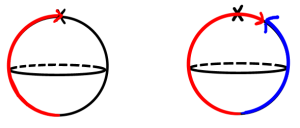
\includegraphics{2019/02/20190221_greatcirclegeodesics.png}
    \caption{Left: a 2-sphere with a geodesic that travels from the south pole to the north pole (marked by an $X$). Right: a 2-sphere with a geodesic (red) that continues through the north pole. As this geodesic has passed through a focal point, it no longer minimizes the distance between its endpoints, and can be deformed into the geodesic in blue which is of shorter length.}
    \label{fig:greatcirclegeodesics}
\end{figure}

Consider now a 2D spacelike surface $S$. We have seen that (in $3+1$ dimensions) we can introduce two future-directed null vector fields (ingoing/outgoing trajectories, if you like) $U^a_1$ and $U^a_2$ on $S$ that are normal to $S$. Consider the null geodesics which have one of these vectors as their tangent on $S$. A point is \term{conjugate} to a surface if there is a Jacobi field which is tangent on the surface and vanishes at that point. The analogue of Thm. \ref{conjugatepoints} is then as follows.

\begin{thm}
    A point $P$ is conjugate to a surface $S$ if $\theta \to -\infty$ at $p$ along one of the geodesics parametrized by $U^a_1,U^a_2$.
\end{thm}

\begin{defn}
    Let $(\cM,g)$ be a time-orientable spacetime $U\subset{ \cM}.$ The \term{chronological future/past} of $U$, denoted $I^\pm(U)$, is the set of points of $\cM$ which can be reached by a future-/past-directed timelike curve starting on $U$ (not including $U$).
\end{defn}
\begin{figure}
    \centering
    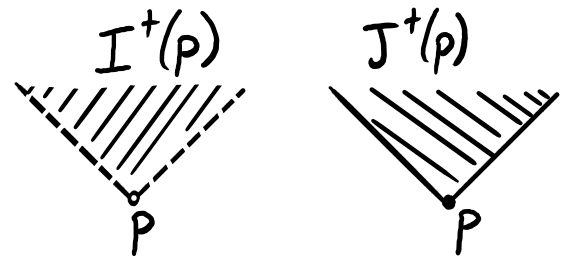
\includegraphics[width=0.5\textwidth]{2019/02/20190221_chronofuture.png}
    \caption{The chronological future $I^+$ and the causal future $J^+$ in Minkowski space. Notice that the chronological future $I^+(p)$ is strictly the interior of the light cone of the point $p$ and does not include $p$ itself, whereas the causal future includes the light cone and $p$ itself.}
    \label{fig:chronofuture}
\end{figure}
\begin{defn}
    The \term{causal future/past} of $U$, denoted $J^\pm(U)$, is the union of $U$ with the set of points of $\cM$ that can be reached by a future-/past-directed \emph{causal} curve starting on $U$.
\end{defn}

\begin{thm}\label{surfaceconjugatepoints}
    Let $S$ be a two-dimensional orientable spacelike submanifold of a globally hyperbolic spacetime $(\cM,g)$. Then every point $p\in \dot J^+(S)$ (the topological boundary of $J^+(S)$) lies on a future-directed null geodesic starting from $S$ which is orthogonal to $S$ and has no point conjugate to $S$ between $S$ and $p$. Furthermore, $\dot J^+(U)$ is a submanifold of $\cM$ and is achronal (no two points on $\dot J^+(U)$ are connected by a timelike curve), where $U\subset \cM$.
\end{thm}
%The topological boundary is the set minus the interior. The interior is the set of points where there exists a neighborhood centered on that point etc
%You might not be familiar [with these topological concepts]. But you need to get familiar because we're going to squeeze physics out of this like there's no tomorrow.